\documentclass{article}

\usepackage{fancyhdr}
\usepackage{extramarks}
\usepackage{amsmath}
\usepackage{amsthm}
\usepackage{amsfonts}
\usepackage[plain]{algorithm}
\usepackage{algpseudocode}
\usepackage{matlab-prettifier}
\usepackage{graphicx}
\usepackage[export]{adjustbox}
%
% Basic Document Settings
%
\lstMakeShortInline[style=Matlab-editor]"

\topmargin=-1in
\evensidemargin=0in
\oddsidemargin=0in
\textwidth=6.5in
\textheight=9.0in
\headsep=0.25in

\linespread{1.1}


\rhead{\firstxmark}
\lfoot{\lastxmark}
\cfoot{\thepage}

\renewcommand\headrulewidth{0.4pt}
\renewcommand\footrulewidth{0.4pt}

%
% Homework Details
%   - Title
%   - Due date
%   - Class
%   - Section/Time
%   - Instructor
%   - Author
%

\newcommand{\hmwkTitle}{AMATH 482 Homework 1: An Ultrasound Problem}
\newcommand{\hmwkDueDate}{January 25, 2019}
\newcommand{\hmwkClassInstructor}{Professor Nathan Kutz}
\newcommand{\hmwkAuthorName}{\textbf{Skyler Hallinan}}

%
% Title Page
%

\title{
    \textmd{\textbf{\text{ } \hmwkTitle}}\\
}

\author{\hmwkAuthorName}
\date{}

\begin{document}
\maketitle

\section*{\fontsize{19}{15}\selectfont Abstract}
	We were given noisy, 3-D ultrasound data taken from our dog's intestine, in the hopes of identifying the path and location of a foreign object. We used the fast fourier transform to move our data to the frequency domain, and determined the frequency signature via averaging the spectrum. We centered a 3-D gaussian filter around these coordinates and multiplied it by the fourier-transformed data. We then transformed back into the space domain, and determined the location of the marble with our now denoised data.
\section*{\fontsize{19}{15}\selectfont Introduction and Overview}
	Our dog Fluffy has swallowed a marble that is currently in the small intestine, but we do not know the location or path of this foreign object. Through ultrasound taken at 20 time points, we have obtained data that show the spatial variations in our data. Due to our dog's movement, there is lots of noise in these measurements. We must determine the location of the marble at the 20th data point to know where to focus an intense acoustic wave and remove the marble. \\ \\
In order to remove noise from the data, we must apply a multidimensional fourier transform across the dataset, which consists of 20 64x64x64 sets of spacial ultrasound data. Then we must find the determine the frequency signature by taking the average of the fourier transforms at the 20 time points, which will remove the white noise, assuming it follows a normal distribution. This will let us  find our central frequency and the location in the frequency domain at which it occurs. We will then need to center a filter around this frequency, multiply it by our fourier-transformed dataset, then convert back into the time domain to denoise our data. With this now denoised spacial ultrasound data, we will be able to determine the location and path of the marble in Fluffy's intestine, and determine the 20th point so that we can remove the marble successfully.
\section*{\fontsize{19}{15}\selectfont Theoretical Background}
	Fourier introduced that a function $f(x)$ can be written as the sum of sines and cosines. This holds even if $f(x)$ is discontinuous: 
	\begin{equation} \label{eq:1}
		f(x) = \frac{a_0}{2} + \sum_{n=1}^{\infty}(a_ncosnx + b_nsinnx) \quad x\in(-\pi,\pi]
	\end{equation}
	This expansion produces $2\pi$ periodic periodic functions because they are constructions of sines and cosines on the interval $(-\pi, \pi]$ \\ \\
	Expanding on this, we have the fourier transform. The fourier transform is an integral transform that decomposes a time defined function into its frequency components. We see that the Fourier transform and its inverse are defined as: \\
	\begin{equation} \label{eq:2a}
		F(k) = \frac{1}{\sqrt2\pi} \int_{-\infty}^{\infty} e^{-ikx} f(x) dx
	\end{equation}
		\begin{equation} \label{eq:2b}
		f(x) = \frac{1}{\sqrt2\pi} \int_{-\infty}^{\infty} e^{ikx} F(k) dk
	\end{equation}
	The fast fourier transform was developed by Cooley and Tukey in 1960 to perform the forward and inverse fourier transform at faster speeds with an operation count of $O(NlogN)$. It has fast speed and high accuracy, and the important detail to attaining this speed is discretizing the range $x \in [-L,L]$ into $2^n$ points. In addition, this algorithm shifts the data so that $x\in [0,L] \rightarrow [-L,0]$ and $x\in [-L,0] \rightarrow [0, L]$, multiplies every other mode by -1, and assumes that the user is working on a $2\pi$ periodic domain. In order to visualize this, one must  use "fftshift" on the data and the axes to undo the shifts naturally incurred by the fast fourier transform algorithm. In addition, multidimensional fast fourier transforms are possible.\\ \\
	Nontrivial noise when trying to detect things is a large issue in data that can be resolved through fourier shifting and filtering. Spectral filtering, where only a particular frequency of interest is chosen to be filtered on, allows for lots of unnecessary data and noise to be filtered out. We have the general gaussian filter for spectral filtering: 
	\begin{equation} \label{eq:3}
	F(k) = exp(-\tau (k-k_0)^2)
	\end{equation}
	where $k$ is the wavenumber and $\tau$ is the bandwidth of the filter. Filters can be used to denoise the system by multiplying on data in the fourier domain, to remove unwanted signal. Then, after transformation back to the space domain, noise will be removed.
\section*{\fontsize{19}{15}\selectfont Algorithm Implementation and Development}
In order to conduct the fast fourier transform, we made sure to discretize our x into 64 points so that it matched the $2^n$ criteria. In addition, we rescaled our wavenumbers $k$ by $\frac{2\pi}{L}$ as the fast fourier transform assumes $2\pi$ periodic signals. We also created a grid by which to visualize the signals with "meshgrid" in both the space and frequency domain. \\ \\
We first reshaped the 20 x 262144 dataset into a 20x64x64x64 one using the "reshape" command. This 4-D array represented 20 different 64x64x64 3-D spatial representations through time. This data was noisy; as Figure 1 shows, there is almost no way to make anything out through all of the noise.  \\ \\
We then applied the n-dimensional fast fourier transform to our data via "fftn". This gave us a 4-D matrix: 20 rows of 64x64x64 fourier-transformed data. Next, we had to average the spectrum in order to remove the white noise from the data. We used a loop to add each of the 20 64x64x64 matrices together to an "avg" matrix, then normalized it by dividing "abs(avg)" by the max of the "abs(avg)". We graphed the "fftshift" of the "avg" matrix, then found the max value and index through the "[M,I] = max(avg)" command. After obtaining the integer index "I", we used "[i,j,l] = ind2sub([64,64,64], I)" to determine the appropriate indeces in "Ks" domain. We then plugged these indeces in to receive the appropriate coordinates; ie, "ks(l)" gave use the z coordinate in the frequency domain of the center frequency. We do note that we had to switch the "ks(i)" and "ks(j)" into the y and x coordinates respectively, due to quirks in MATLAB.  \\ \\
Finally, with the coordinates of the central frequency of the fftshifted fourier-transformed "avg" matrix, we created a 3-D gaussian filter centered around that point, choosing a specific $\tau$ value. We ifftshifted this gaussian filter (as we generated it in the fftshifted domain), multiplied our 4-D matrix by it, then used "ifftn" to convert this whole 4-D, 20x64x64x64 matrix back into the space domain. After this, we determined the max coordinate of each of the 20 64x64x64 denoised spacial datsets (which represented the point of the marble at that time point) and used "isosurface" and "plot3" to visualize the marble through time.

\begin{figure}[H]
\begin{center}
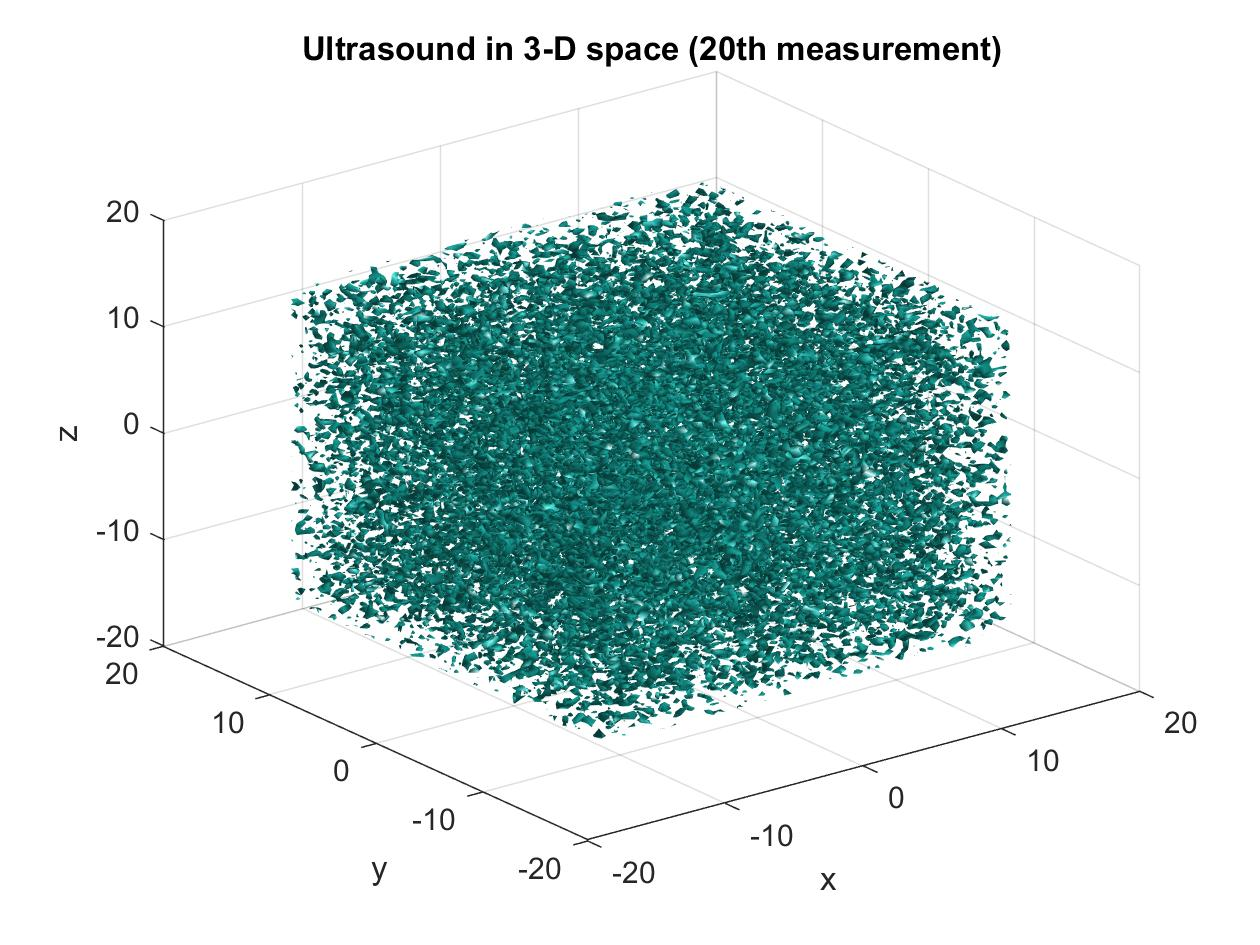
\includegraphics[width = 8cm]{sample3d}
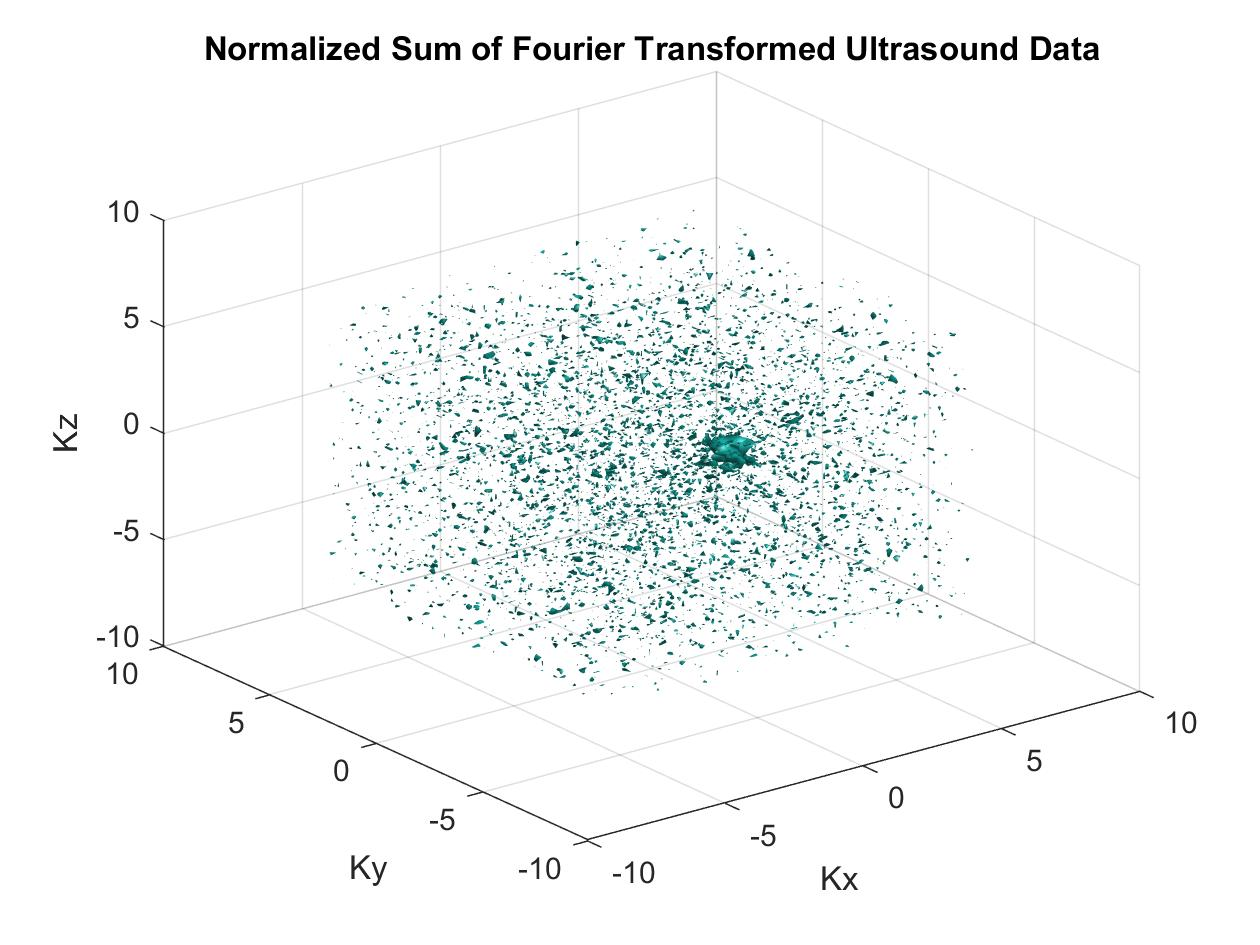
\includegraphics[width = 8cm]{fourieravg}
\caption{\label{fig:scaled_diss} (left) 3-D isosurface plot in space of the ultrasound at the 20th time point. Isovalue of 0.75.}
\caption{\label{fig:scaled_diss} (right) 3-D isosurface plot in frequency domain of normalized, averaged fourier-transformed data. Isovalue of 0.725.}
\end{center}
\end{figure}

\section*{\fontsize{19}{15}\selectfont Computational Results}
	After summing each of the 20 fourier-transformed 64x64x64 matrices into an "avg" matrix and normalizing, we plotted the "fftshift" of this on the frequency domain. Figure 2, shows our normalized fourier-transformed average data, and there appears to be a clear central frequency, taking the form of the blob in the figure. We determined the coordinates of this central frequency, to be at the coordinate $(1.8550, -0.8378, 0)$ on the Kx, Ky, Kz grid. \\ \\
We then centered our 3-D gaussian filter around this coordinate, and generated the following 3-D gaussian filter: "exp(fwid*(Kx - cx).^2 +fwid*(Ky - cy).^2 + fwid*(Kz - cz).^2)" where "cx", "cy", and "cz" are 1.8850, -0.3878, and 0, and where our $\tau$ value in the general gaussian filter equation was "fwid = -0.5" (we used a negative here for simplicity in multiplication. $\tau$ is usually positive). We tried a variety of $\tau$ values, and found that there was generally a large range that worked (0.1 to 2); however, at too small $\tau$ values, there still appeared to be lots of noise in the data, and at $\tau$ values to high, our isosurface graph and 3-D plot in time graphs became unreadable. \\ \\
After multiplying the "ifftn" of this filter to each of the 20 fourier-transformed 64x64x64 data, we took the ifftn of the entire 4-D dataset, and plotted it with "isosurface". We obtained Figure 3, which shows a clear path and shape of the marble through time, as the data is now denoised. In addition, we generated Figure 4, which shows the path of the marble in the form of a line graph. Through these we determined that the 20th point, the marble was at location $(-5.1563, 4.2188, -6.0938)$.


\begin{figure}[H]
\begin{center}
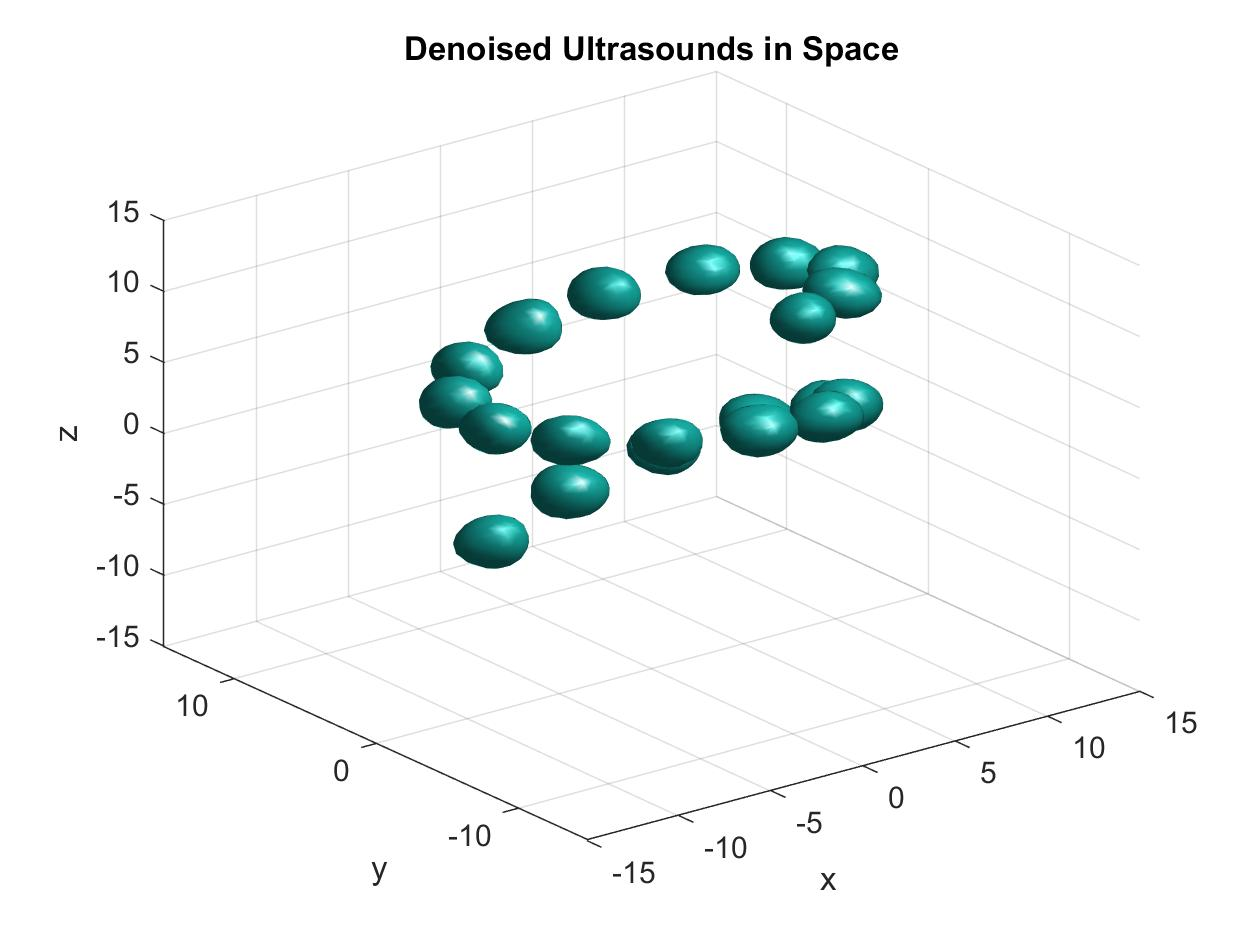
\includegraphics[width = 8cm]{denoised3d}
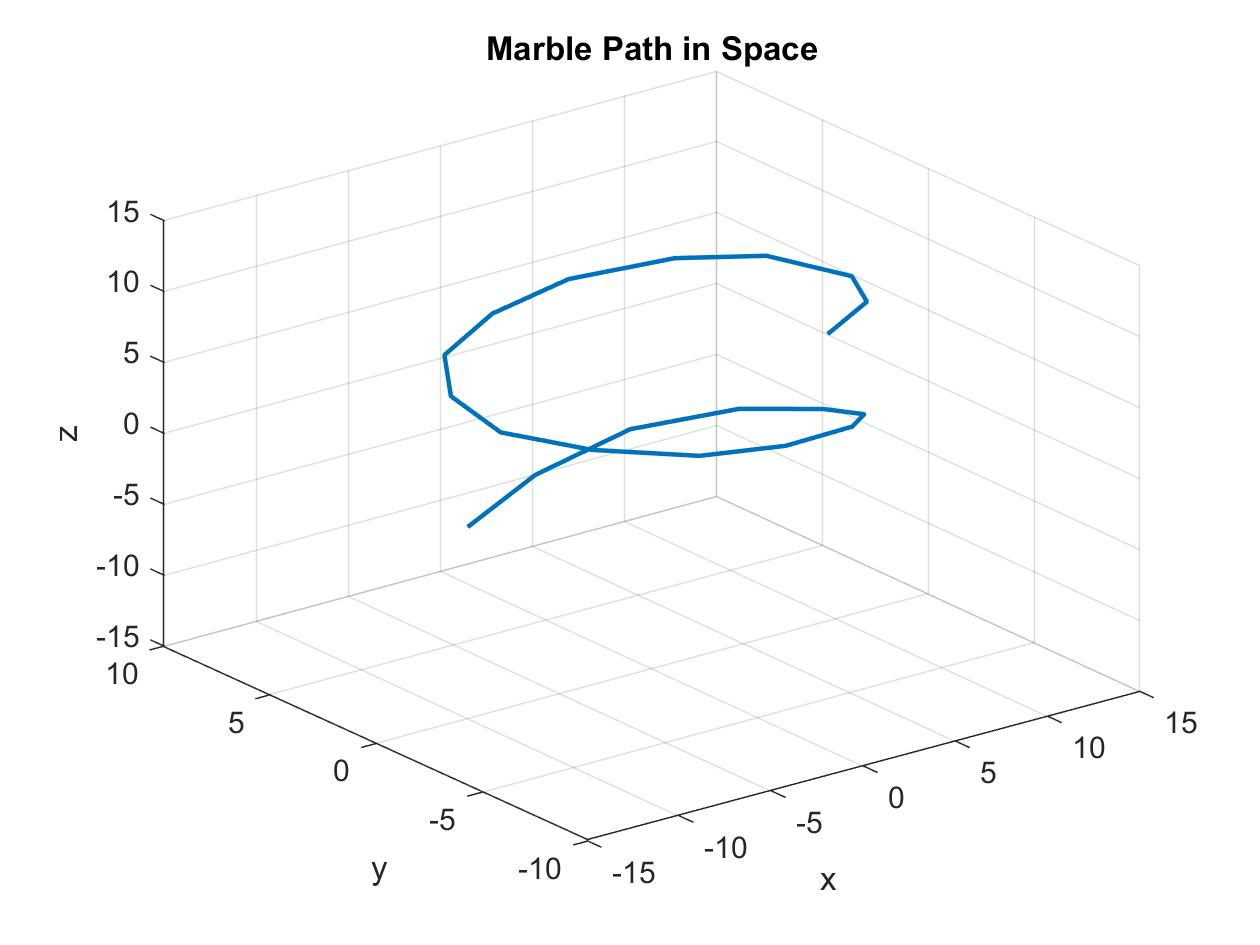
\includegraphics[width = 8cm]{marblepath}
\caption{\label{fig:scaled_diss} (left) 3-D isosurface plot in space of the denoised marble. Isovalue of 0.6.}
\caption{\label{fig:scaled_diss} (right) 3-D plot in space domain of marble path.}
\end{center}
\end{figure}

\section*{\fontsize{19}{15}\selectfont Summary and Conclusions}
We started with noisy spatial ultrasound data through time and were trying to determine the location of a marble in our dog's intestine. We located the coordinates of the central frequency at $(1.8550, -0.8378, 0)$ via averaging the spectrum of 20 64x64x64 fourier-transformed datasets. We then generated a filter with a $\tau$ value of 0.5 that we shifted and multiplied by the fourier-transformed 4-D matrix. With this denoised data, we were able to locate the marble in our dog's intestine at $(-5.1563, 4.2188, -6.0938)$ . Based on our results, we suggest to focus the intense acoustic wave at the location of $(-5.1563, 4.2188, -6.0938)$ (in the x, y, z space domain) in order to remove the marble and save Fluffy. 
\pagebreak




\section*{\fontsize{19}{15}\selectfont Appendix A}
\subsection*{MATLAB functions used and implementation}
"abs(X)" : Returns the absolute value of every element in X, or complex magnitude if the element is complex. We used this function to normalize the data by dividing "abs(X)" with the max of "abs(X(:))", where X was a 64x64x64 matrix. \\ \\
"[i,j,k] = ind2sub(siz,IND)" : Given a index "IND", it returns the "i", "j", and "k" indeces, which can then be translated into spacial or frequency domain coordinates. We used this command to find the center frequency of our averaged spectrum, and the location of the marble throughout time in the space domain via our denoised data. \\ \\
"fftn(X)" : Performs a multidimensional fast fourier transform on "X", an N-D array. We used this fourier transform on our 20x64x64x64 ultrasound data to transform into the frequency domain. \\ \\
"fftshift(X)" : Rearranges the contents of "X" by placing the zero-frequency component to the center of the array. If "X" is a vector, shifts the left and right halves of "X", while if "X" is a matrix, the $I$ and $III$ quadrants are switched, as well as the $II$ and $IV$ quadrants. We used this to change our transformed data and our axes for proper visualization, with "isosurface" and such.  \\ \\
"ifftn(X)" : Performs a multidimensional discrete inverse fast fourier transform on "X". We used this after multiplying our centralized filter on the fourier-transformed data to transform it back into the spacial domain as denoised data.\\ \\
"ifftshift(X)" : Performs the inverse of "fftshift(X)". We used this on our filter to undo the "fftshift" that had been done when creating the filter. \\ \\
"isosurface(X,Y,Z,V,isovalue)" : Computes and plots the isosurface from volume data "V" at the isosurface value "isovalue". We used this to visualize the ultrasounds at different times in the spatial and frequency domain.\\ \\
"linspace(x1,x2,n)" : Creates a vector of "n" evenly spaced points from "x1" to "x2". We used this to create a linearly spaced vector in the spacial domain, which we then used for the "meshgrid".  \\ \\
"[X,Y,Z] = meshgrid(x,y,z)" : Creates 3-D grid coordinates defined by the "X", "Y", and "Z" vectors. We used this to define axes to plot isosurfaces in the space and frequency domains.\\ \\
"max(A)" : If "A" is a vector, then it returns the maximum value of this vector. We used this for normalization of data. \\ \\
"[M,I] = max(A)" : Returns the maximum value "M" and the index "I"  of the matrix, which we then used in "ind2sub" to find direct coordinates.  \\ \\
"plot3(X1,Y1,Z1)" : Displays a 3-dimensional plot of a set of datapoints through inputs "X1", "Y1", "Z1". We used this to visualize the path of the marble in the intestine after noise was removed and 20 data points were obtained in 3-dimensional space. \\ \\
"reshape(A,sz)" : Reshapes the array "A" to the size defined by "sz". We used this to store the initial data as a 4-D 20x64x64x64 matrix. We also used this command to access each row of this 4-D matrix for plotting, etc. \\ \\
"zeros(A,B,C)" : Creates a matrix filled with zeros of size "A x B x C". We used this to initialize an average matrix, where we stored and added 20 64x64x64 fourier transformed matrices together. \\ \\

\section*{\fontsize{19}{15}\selectfont Appendix B}
\subsection*{MATLAB code}
\begin{lstlisting}[style=Matlab-editor]
clear all; close all; clc;
load Testdata

L=15; % spatial domain
n=64; % Fourier modes

x2=linspace(-L,L,n+1); x=x2(1:n); y=x; z=x;
k=(2*pi/(2*L))*[0:(n/2-1) -n/2:-1]; ks=fftshift(k);
[X,Y,Z]=meshgrid(x,y,z);
[Kx,Ky,Kz]=meshgrid(ks,ks,ks);

figure
Un(:,:,:)=reshape(Undata(20,:),n,n,n);
isosurface(X,Y,Z,abs(Un), 0.75)
axis([-20 20 -20 20 -20 20]), grid on, drawnow
xlabel("x"), ylabel("y"), zlabel("z")
title("Ultrasound in 3-D space (20th measurement)")

Undatashape = reshape(Undata, [20,n,n,n]);
Ut= fftn(Undatashape);
avg = zeros(64,64,64);
for p = 1:20
    avg(:,:,:) = avg + abs(reshape(Ut(p,:),n,n,n));
end
avg = avg./20;
avg = abs(avg)/max(abs(avg(:)));

figure
isosurface(Kx,Ky,Kz,fftshift(avg), 0.725)
axis([-10 10 -10 10 -10 10]), grid on, drawnow
xlabel("Kx"), ylabel("Ky"), zlabel("Kz")
title("Normalized Sum of Fourier Transformed Ultrasound Data")

avgshift = fftshift(avg);
[maximum, index] = max(avgshift(:));

[ii,jj,ll] = ind2sub([n,n,n], index);

cx = ks(jj); cy = ks(ii); cz = ks(ll);
%%
fwid = -0.01;
filter = exp(fwid*(Kx - cx).^2 +fwid*(Ky - cy).^2 + fwid*(Kz - cz).^2);

for j=1:20
    Uncur(:,:,:)= reshape(Ut(j,:),n,n,n);
    filterall(j,:,:,:) = ifftshift(filter).*Uncur;
    close all, isosurface(Kx,Ky,Kz,abs(fftshift(Utfn)), 0.5)
    axis([-20 20 -20 20 -20 20]), grid on, drawnow
end

figure;
Undenoise = ifftn(filterall);
for j = 1:20 
    Unslice(:,:,:)= reshape(Undenoise(j,:),n,n,n);
    Unslice = abs(Unslice)/max(abs(Unslice(:)));
    [maximum, index] = max(abs(Unslice(:)));
    [ii,jj,ll] = ind2sub([n,n,n], index);
    plotdata(j,:) = [X(ii,jj,ll),Y(ii,jj,ll),Z(ii,jj,ll)];
    isosurface(X,Y,Z,abs(Unslice), 0.6)
    axis([-20 20 -20 20 -20 20]), grid on, drawnow
end
xlabel("x"), ylabel("y"), zlabel("z")
title("Denoised Ultrasounds in Space");

figure;
plot3(plotdata(:,1), plotdata(:,2), plotdata(:,3), "Linewidth", 1.5)
axis([-15 15 -10 10 -15 15]), grid on, drawnow
xlabel("x"), ylabel("y"), zlabel("z")
title("Marble Path in Space");

point = plotdata(20,:)
\end{lstlisting}

\end{document}
